% neginhib cogsci submission


\documentclass[10pt,letterpaper]{article}

\usepackage{cogsci}
\usepackage{pslatex}
\usepackage{apacite}
\usepackage{graphicx}

\title{inhibition, negation and implicature processing}
 
\author{{\large \bf Ann E. Nordmeyer} \\
  \texttt{anordmey@stanford.edu} \\
  Department of Psychology \\
  Stanford University
  \And {\large \bf Erica J. Yoon} \\
  \texttt{ejyoon@stanford.edu} \\
  Department of Psychology \\
  Stanford University
  \And {\large \bf Michael C. Frank} \\
  \texttt{mcfrank@stanford.edu} \\
  Department of Psychology \\
  Stanford University}

\begin{document}

\maketitle


\begin{abstract}

...

\textbf{Keywords:} 
Inhibitory control; negation; implicature; drift diffusion model; cognitive development; pragmatics

\end{abstract}


\section{Introduction}

Previous research has shown that children have a hard time processing negation \cite{nordmeyer2014role} and implicature \cite{yoonchildren}. One possible reason is inhibitory demand of these processes, rather than the lack of pragmatic understanding, which children demonstrate from an early age (e.g., \citeNP{katsos2011pragmatic, matthews2012two}).

The current study uses a simple game with three phases that test children's processing of inhibitory demands, negation and implicature, respectively. We used nearly identical auditory and visual stimuli for the three phases, which allowed direct comparisons. % of... 

We use the drift diffusion model \cite{ratcliff1978theory} to look at the deeper meanings of behavioral responses that may look similar on surface. We also compare our data with a previous diffusional model analysis of developmental changes in a different cognitive task \cite{ratcliff2012children} and show our results align.  AEN.NOTE: explain DDM in some detail here, or in beginning of results section?

We also compared performances on tablet vs. computer, which will be informative for future studies that use these tools.

\section{Method}

\subsection{Participants}

We invited children at Bing Nursery School at Stanford University and Children'��s Discovery Museum in San Jose, CA, to play a game to find things that are named. 4-year-olds (N = FIXME; M = FIXME) played the game on an iPad, and 4-, 5-, and 6-year-olds played the game on a computer (N = FIXME respectively; M = FIXME respectively). (FIXME: exclusion criteria?) We also recruited adult participants (N = FIXME) on Amazon Mechanical Turk to play the computer version of the task.  

\subsection{Stimuli and Design}

AEN.NOTE: I think we should introduce "target" vs. "control" conditions here (i.e. what we mean by that in each game) so that we can use these terms in the results section.

The game consisted of three phases that each tested one of the target processes: inhibition, negation processing, and implicature processing. In each trial in all three phases, there were two images side-by-side on the screen. a Pre-recorded voice said one or two words to refer to the target image, and participants' task was to select the correct referent as soon as they could identify it.

For the ``inhibition'' phase, in a set of 6-8 trials, the same two pictures appeared together (e.g., a picture of a carrot and a picture of a banana), with randomized sides. For the first 5-7 trials ({\emph control}), the same object was named (e.g., ``carrot''), then on the last trial  ({\emph inhibition}), the other object was named (``banana''). Participants were predicted to gain speed on every trial until the last one, in which the accuracy rate was expected to fall, due to the inhibitory demand. Child participants saw a total of 12 sets of trials, and adults saw 24 sets, in the inhibition phase.

For the ``negation'' phase, the referents were named with or without negation. For example, given two pictures of carrot and banana respectively, to refer to the banana the recorded voice said ``banana'' (in a {\emph positive} trial) or ``no carrot'' (in a {\emph negative} trial). Children saw 60 trials, and adults saw 120 trials in the negation phase. 

For the ``implicature'' phase, in each trial there was a picture with one object (e.g., carrot) and another picture with the same object and another one (e.g., carrot and banana). In an {\emph unambiguous} trial, the unique object was named (``banana'') and in an {\emph implicature} trial, the common object was named (``carrot''), implying ``carrot {\emph but not banana''}. Children saw 60 trials, and adults saw 120 trials in the implicature phase. 

\subsection{Procedure}

Adult participants first went through two practice trials, where they were asked to select an obvious, unambiguous referent (e.g., ``cow'' as opposed to ``rabbit''). Then they went through the three test phases in a randomized order.

For child participants, an experimenter first explained the game. Then, for those participants playing the computer version, it proceeded in the same way as for adult participants. For participants playing the iPad version, they played a dots game, where they tapped five dots in random locations, which helped them practice using the iPad screen. Once participants were used to using the screen, they proceeded to the test phases. After the child participants were finished, the experimenter gave them a sticker as a gift and thanked them for playing the game.

\section{Results and Discussion}
AEN.NOTE: do you think we need to talk about traditional RT analyses too?  They're just so boring/unclear for these data so I'm inclined to skip this, but it might seem like a gap to reviewers.  One thing that I was thinking is that we could say something about pilot data suggesting few differences in RT data, which is why our planned analysis for this study was the drift diffusion model?  Or we could very briefly discuss RT and accuracy differences (or lack thereof) in the adult data, without showing any plots, and then move on to the DDM analysis for adults and kids.

AEN.NOTE: I need to go back through and get terminology consistent (e.g. condition vs. trial type)

We fit the diffusion model separately to each individual participant's data using the RWiener pakage\footnote{All analyses described in this paper were conducted using R version 3.2.1}, which uses the Nelder-Mead method to estimate optimal parameter values.  We estimated parameters separately for each condition (target vs. control) within each game, and calculated the mean and 95\% C.I. across all participants within each age group (4-year-olds, 5-year-olds, 6-year-olds, and adults).  We then used these parameter estimates to produce visualizations of the decision process for each condition across each game and age group (see Figures \ref{fig:adults} and \ref{fig:kids}), allowing us to compare the diffusion process across the three games, as well as across the four age groups.  

\subsection{Differences across games}

\begin{figure*}
\begin{center} 
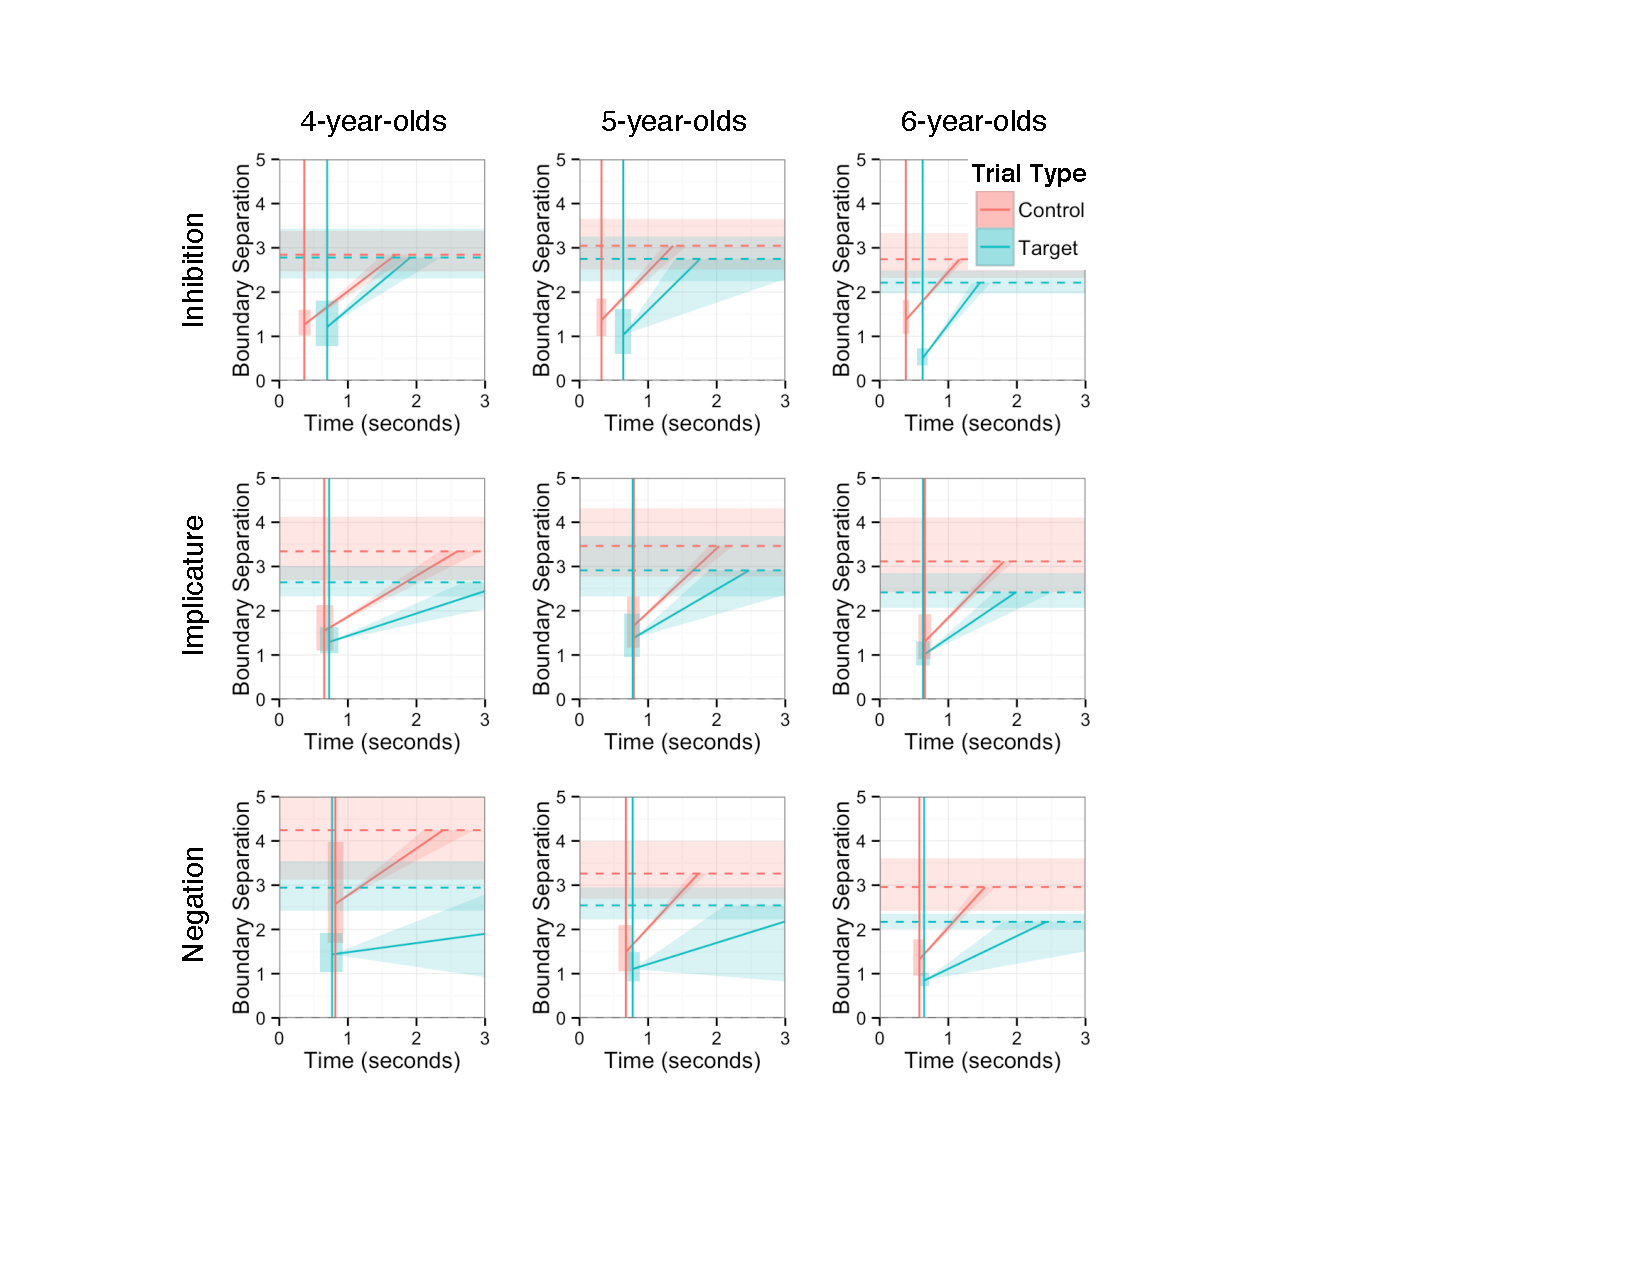
\includegraphics[width=6in]{figures/adult_vis.pdf}
\caption{\label{fig:adults} Visualization of the drift diffusion process for adults across the three games.  The process for control trials is shown in pink, and the process for target trials is shown in green.  The dotted black line at zero represents the threshold for making an incorrect decision, and horizontal colored lines represent the boundary separation parameter (i.e. the threshold for making a correct decision).  Vertical colored lines represent the non-decision time parameter, and the slope of the decision process (angled line) represents the drift rate parameters.  The point where the decision process intercepts the non-decision line represents the bias $\times$ boundary separation.  Ribbons around all lines represent 95\% confidence intervals around each parameter.}
\end{center} 
\end{figure*}

First we explored similarities and differences in the decision process for adults across each of the three games.  We hypothesized that there might be similar process for these three games, because the target trials for each game involve selecting an image that is less salient or interesting for participants.  In Figure 1, we plot the decision process for each of these three games.  Surprisingly, despite the surface similarities of these games, the decision process for control vs. target trials appears to be different across the three games.  In the inhibition game, the most striking difference between control and target (inhibition) trials is the bias towards incorrect trials on target trials.  In the implicatures game, the most striking difference between control (unambiguous) and target (implicature) trials is the higher boundary separation but faster drift rate for control trials compared to target trials.  In the negation game, there appears to be little difference in the decision process between control (positive) and target (negative) trials.

We conducted post-hoc paired t-tests to compare parameter values for control vs. target trials in each game.  In the inhibition game, the bias parameter was significantly lower (e.g. biased towards the incorrect trial) for target trials compared to control trials (STATS).  In the implicature game, the boundary separation and the drift rate was significantly higher for control trials compared to target trials (Boundary Separation: STATS; Drift: STATS).  For the negation game, there was no significant difference between drift rate for control vs. target trials.  

Although we were surprised by the striking differences across the three games, the decision process that we do see makes sense within the context of each game.  For example, we would expect target trials in the inhibition game to be biased towards incorrect trials, because the game is intentionally designed to create such a bias.  Similarly, the slower drift rate for target trials in the implicatures game makes sense, because these trials are ambiguous (either picture is technically correct), so participants take longer to accumulate enough information to resolve this ambiguity.  The most surprising finding was the lack of difference between positive and negative trials in the negation game.  Past work suggests that adults take longer to respond to negative sentences compared to positive ones (CITE), especially in context-free tasks such as this (CITE).  One possibility is that the high number of repeated trials, or the simplistic and child-friendly stimuli, made this task easier for adults.

\subsection{Developmental differences}

\begin{figure*}
\begin{center} 
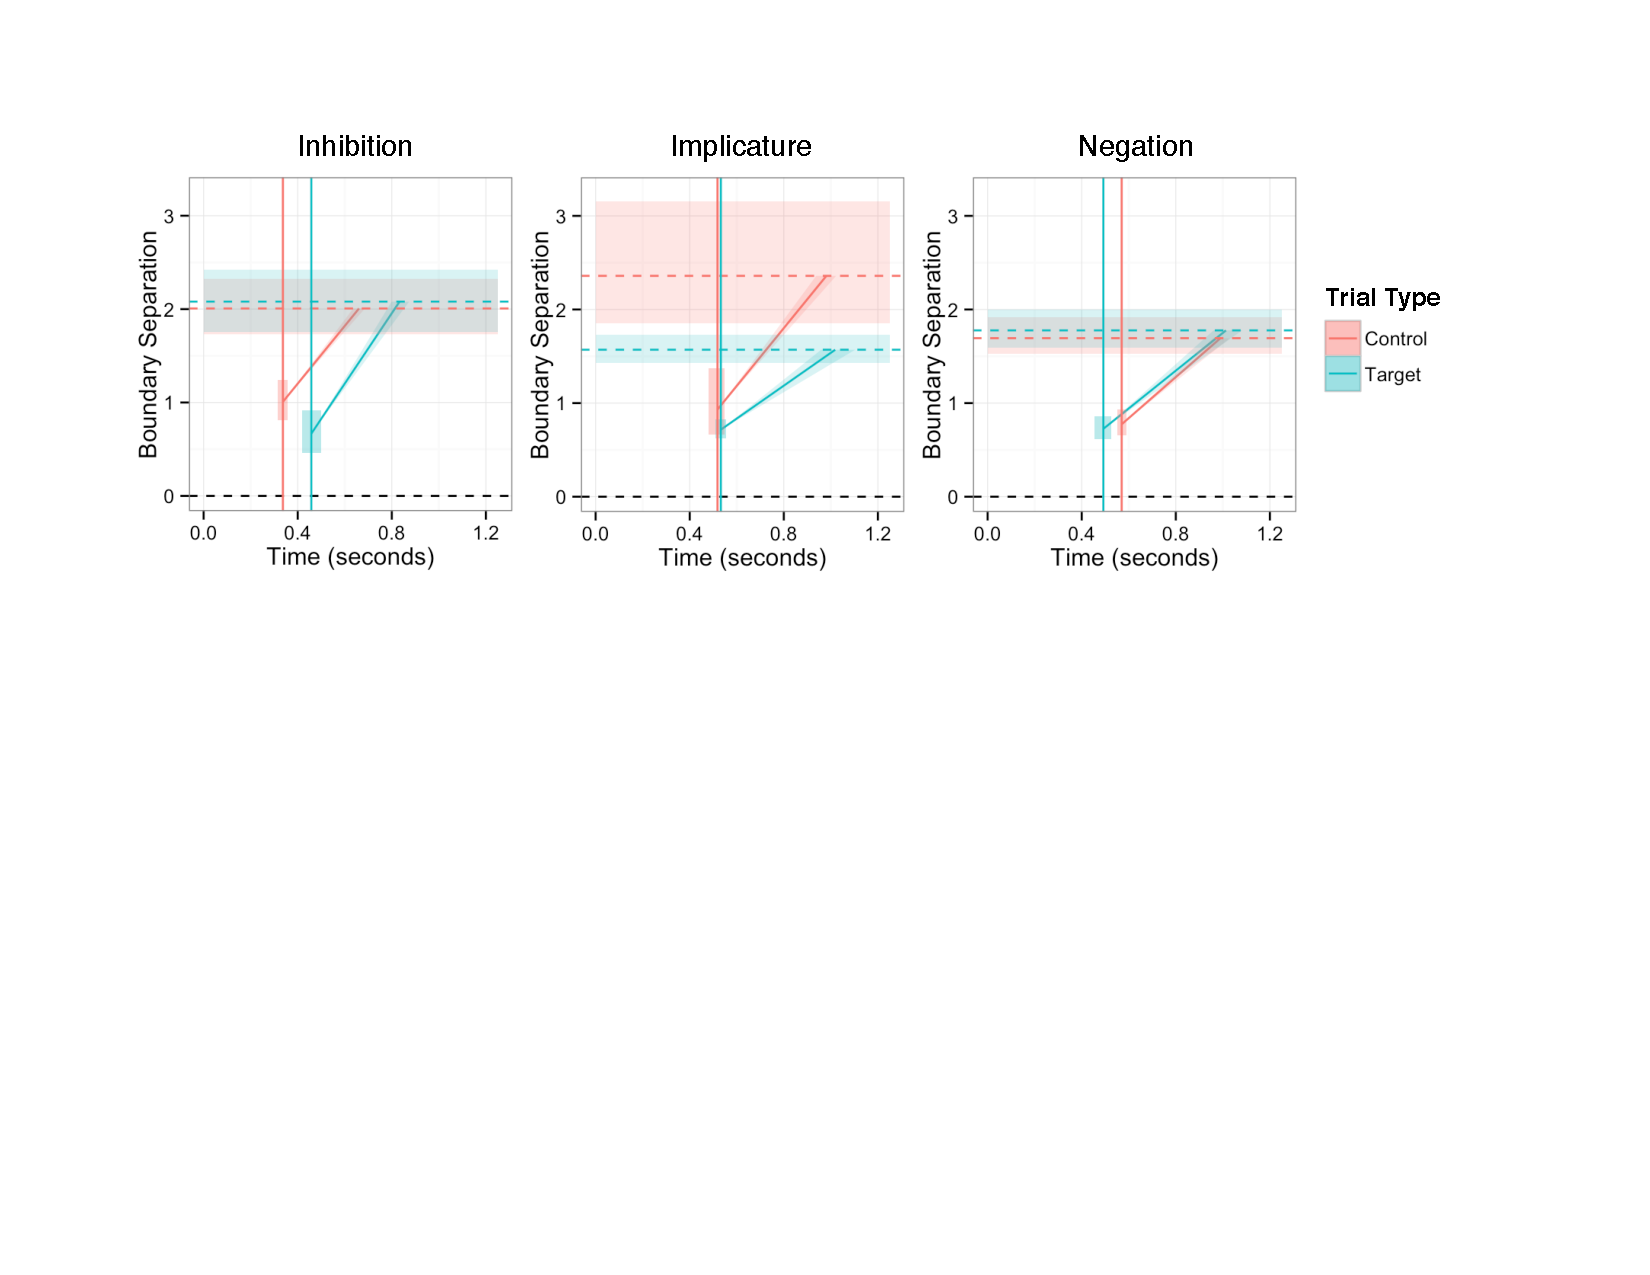
\includegraphics[width=6in]{figures/child_vis.pdf}
\caption{\label{fig:kids} Visualization of the drift diffusion process for 4-year-olds, 5-year-olds, and 6-year-olds across the three games.  Plotting conventions are the same as in Figure \ref{fig:adults}.}
\end{center} 
\end{figure*}

Next we explored developmental change in preschoolers between 4 and 7 years of age.  The decision process for each game across the three age groups is visualized in Figure \ref{fig:kids}.  For the inhibition and implicature games, children at all ages look similar to adults, with developmental change across the three age groups as children's decision process gets more adult-like.  For example, in the inhibition game, 4-year-olds are actually \emph{less} likely to show a bias towards the incorrect trial; this bias appears to get stronger by age 6.  In the implicatures game, children have a slower drift rate for target trials compared to control trials even at age 4, but this difference becomes more striking as children get older.  The most striking difference between children and adults is in the negation game, where the drift rate for target trials is dramatically slower compared to control trials, although developmental change is evident in this game as well.  

To examine the reliability of our findings, we fit linear mixed-effects model to the data for each of the three games to explore how the interaction between condition (control vs. target trials) and age group influences different parameters.  For the inhibition game, we see a significant interaction between age group and trial type for four-year-olds (STATS) and a marginally significant interaction for five-year-olds (STATS), indicating that for four and five-year-olds the bias parameter for target trials in the inhibition game is higher compared to adults.  There is no interaction between age group and condition for six-year-olds, supporting that six-year-olds are more adult-like in their bias towards the incorrect trial on the inhibition game.

For the implicatures game, we found a main effect of age group, with a significantly slower drift rate overall for four, five, and six-year-olds.  There was also a significant interaction between age group and trial type for four, fives, and six-year-olds, indicating that the difference between drift rate for target vs. control trials is much smaller for children compared to adults (STATS).  We found the opposite pattern in the negation game: Although there was a similar main effect of age group, with children showing significantly slower drift rates overall compared to adults (STATS), children at all age groups showed a \emph{greater} difference in drift rate between control and target trials compared to adults, as indicated by significant negative interactions between age group and trial type for all age groups (STATS).  

We can also use our data to look at overall changes in the decision process across age groups, regardless of the task that children were engaged in. Across all three games, children at all age groups had higher boundary separation parameters (STATS) and longer non-decision times (STATS compared to adults.  Children also had significantly slower drift rates compared to adults, with drift rate changing significantly even across ages 4 to 6 (STATS).  These data replicate past findings from (CITE the ratcliff cdev paper we read in lab meeting), which found similar differences between adults and elementary-school aged children, with a much younger sample of children.  Furthermore,  the finding that drift rate increases in our tasks from age 4 to age 6 suggests that changes in the speed at which children accumulate evidence changes rapidly in early childhood.  (AEN.NOTE: Is this worth keeping in?  I think it's a cool extension of the other developmental ddm paper, but it isn't really theoretically relevant to the inhibition stuff).  




\section{Discussion}

%\section{Acknowledgments}
%
%Bing Nursery School, CDM, Stephen Powell, Veronica, Rachel

\bibliographystyle{apacite}

\setlength{\bibleftmargin}{.125in}
\setlength{\bibindent}{-\bibleftmargin}

\bibliography{neginhib}


\end{document}
